\documentclass[12pt]{article}
% Packages
\usepackage[utf8]{inputenc}
\usepackage{amsmath, amssymb, amsthm}
\usepackage{booktabs}
\usepackage{geometry}
\geometry{margin=1in}
\usepackage{fancyhdr}
\usepackage{enumitem}
\usepackage[most]{tcolorbox}
\usepackage[useregional]{datetime2}
\usepackage{graphicx}
\usepackage{float}

\title{NBA Stats}
\author{Tony Lai}
\date{May 2026}

\begin{document}

\maketitle
\section*{Introduction}

This project studies whether heavier recent playing time is associated with worse current-game performance for NBA players. The data come from NBA regular-season player-game records from the 2021--22, 2022--23, and 2023--24 seasons. The original database reference is Wyatt Walsh's Basketball Dataset on Kaggle, and the project repository stores cached player-game logs used for the analysis.

A player-season was included if the player averaged at least 20.0 minutes per game and appeared in at least 60 games. For each qualifying player-game, the project kept the player name, season, game date, minutes played, and Game Score. Game Score is a box-score performance measure that combines scoring, efficiency, rebounds, assists, steals, blocks, and turnovers into one number.

The explanatory variable is the total number of minutes the player played in the previous five games from the same season. The response variable is Game Score in the current game. The first five games of each player-season were removed because those games do not have five previous games available. This created 34,831 usable player-game observations from 37,441 raw player-game rows.

For inference, the project used a random sample of the full usable data set. Each player-season was treated as a stratum; within each stratum, usable games were split into non-overlapping blocks of five consecutive player-game rows. The sampling procedure randomly selected 40 player-season strata, then randomly selected one five-game block from each chosen stratum using random seed 2789. This produced 40 blocks and 200 sampled player-game observations.

\section*{Variables}

\begin{center}
\begin{tabular}{ll}
\toprule
Variable & Description \\
\midrule
$X$ & Minutes played in the previous five games \\
$Y$ & Current-game Game Score \\
\bottomrule
\end{tabular}
\end{center}

\section*{Sample of the Data Set}

The full sampled CSV has one row for each sampled player-game. The table below shows one complete five-game block for Avery Bradley, so it shows how the main columns of the sampled data set are organized.

\begin{table}[htbp]
\centering
\caption{Example of one sampled non-overlapping five-game block from the data set.}
\label{tab:one-player-sample}
\resizebox{\textwidth}{!}{%
\begin{tabular}{llrlrrrrr}
\toprule
Block ID & Player ID & Player & Season & Game No. & Date & MP & Prev. 5 MP & Game Score \\
\midrule
block\_25\_bradlav01\_2022\_chunk\_04 & bradlav01 & Avery Bradley & 2022 & 21 & 2021-11-28 & 18.3 & 118.7 & -0.9 \\
block\_25\_bradlav01\_2022\_chunk\_04 & bradlav01 & Avery Bradley & 2022 & 22 & 2021-12-07 & 24.5 & 110.6 & 1.5 \\
block\_25\_bradlav01\_2022\_chunk\_04 & bradlav01 & Avery Bradley & 2022 & 23 & 2021-12-09 & 28.7 & 109.0 & 11.3 \\
block\_25\_bradlav01\_2022\_chunk\_04 & bradlav01 & Avery Bradley & 2022 & 24 & 2021-12-10 & 26.4 & 107.8 & 19.6 \\
block\_25\_bradlav01\_2022\_chunk\_04 & bradlav01 & Avery Bradley & 2022 & 25 & 2021-12-12 & 28.7 & 109.6 & 1.6 \\
\bottomrule
\end{tabular}
}
\end{table}

\section*{Hypotheses}

The project tests whether heavier recent workload is associated with lower current-game performance. The regression model is

\[
Y = \beta_0 + \beta_1X + \epsilon.
\]

The hypotheses are

\[
H_0: \beta_1 = 0
\]

\[
H_a: \beta_1 < 0.
\]

\section*{Technical Calculation Method}

The calculations were completed in Python using the project script \texttt{make\_data\_display.py}. The script used \texttt{pandas} to load and clean the player-game data, group games by player-season, create game numbers, and calculate each player's previous five-game minutes. It used \texttt{numpy} to run the least-squares regression and calculate residual-based statistics. The graphs were made with \texttt{matplotlib}.

For the regression, the script used the following least-squares formulas:

\[
b_1 = \frac{\sum (x_i-\bar{x})(y_i-\bar{y})}{\sum (x_i-\bar{x})^2}
\]

\[
b_0 = \bar{y} - b_1\bar{x}.
\]

After finding the regression line, each residual was calculated as

\[
e_i = y_i - \hat{y}_i.
\]

Then the script calculated the sum of squared errors, the residual mean square error, the standard error of the slope, and the test statistic:

\[
SSE = \sum e_i^2
\]

\[
MSE = \frac{SSE}{n-2}
\]

\[
SE_{b_1} = \sqrt{\frac{MSE}{\sum (x_i-\bar{x})^2}}
\]

\[
t = \frac{b_1 - 0}{SE_{b_1}}.
\]

The degrees of freedom for this regression test are

\[
df = n - 2 = 200 - 2 = 198.
\]

\section*{Sample Inference Calculation}

The sample slope was $b_1 = 0.104427$. The standard error of the slope was approximately

\[
SE_{b_1} \approx \frac{0.104427}{5.804} \approx 0.01799.
\]

Using the null hypothesis value $\beta_1 = 0$, the test statistic is

\[
t = \frac{0.104427 - 0}{0.01799} \approx 5.804.
\]

Because the alternative hypothesis is left-tailed, $H_a: \beta_1 < 0$, a large positive test statistic does not support the claim that the true slope is negative. The left-tailed $p$-value is approximately 1, so the result is not statistically significant evidence for the fatigue hypothesis.

\section*{Sample Regression Results}

Using the 200 sampled player-game observations, the least-squares regression line was

\[
\widehat{\text{Game Score}} = -4.0409 + 0.104427(\text{previous five-game minutes}).
\]

\begin{center}
\begin{tabular}{lr}
\toprule
Statistic & Value \\
\midrule
Sample size & 200 player-games \\
Blocks sampled & 40 five-game blocks \\
Slope & 0.104427 \\
$t$ statistic & 5.804 \\
Degrees of freedom & 198 \\
One-sided $p$-value for $H_a: \beta_1 < 0$ & approximately 1 \\
$R^2$ & 0.1454 \\
\bottomrule
\end{tabular}
\end{center}

\begin{figure}[H]
\centering
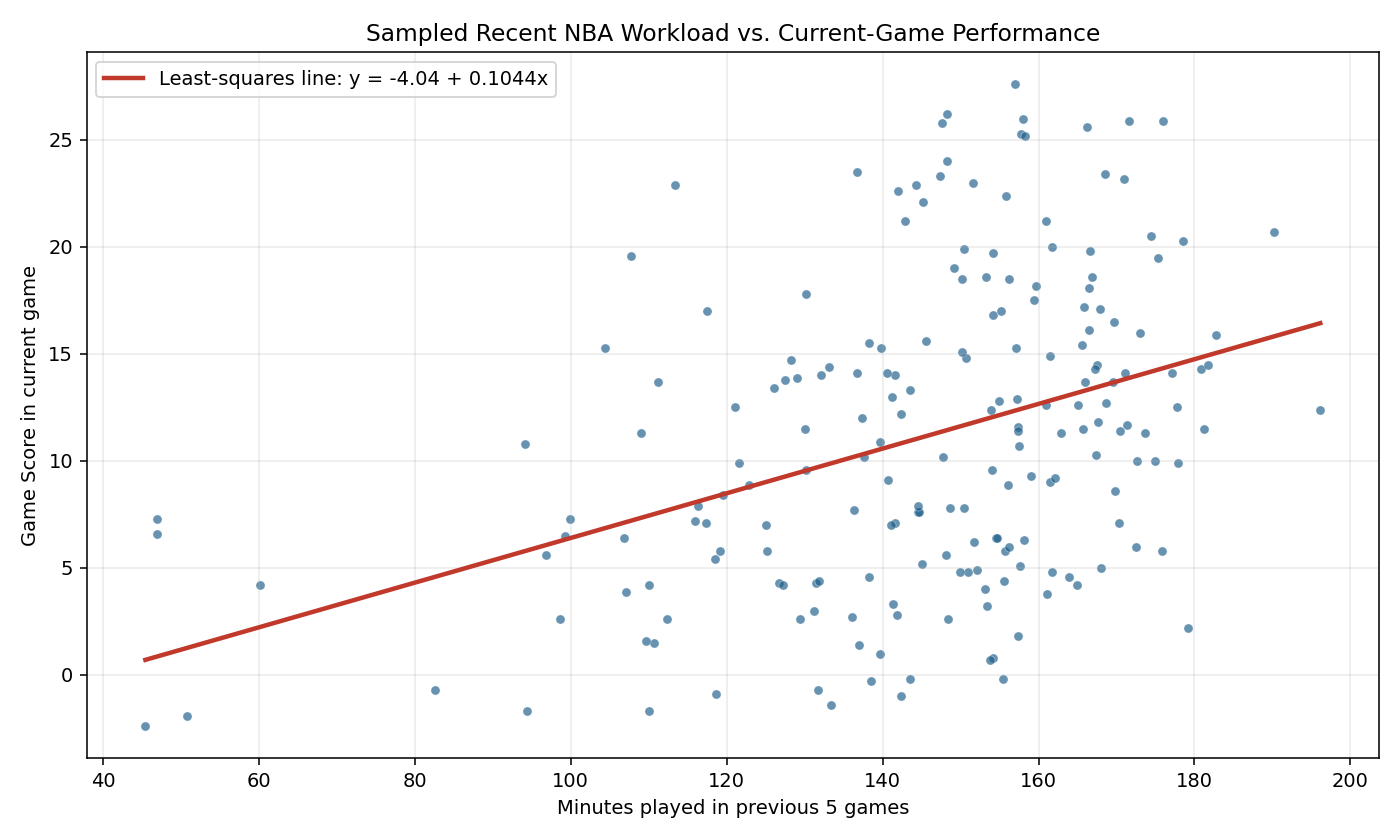
\includegraphics[width=0.88\linewidth]{sampled_workload_scatterplot.png}
\caption{Sampled previous five-game minutes versus current-game Game Score.}
\end{figure}

\section*{Conditions for Regression Inference}

\subsection*{Linear}

The scatterplot shows an approximately linear positive trend between previous five-game minutes and current-game Game Score. The residual plot does not show a strong curved pattern, so the linear condition is reasonably met.

\begin{figure}[H]
\centering
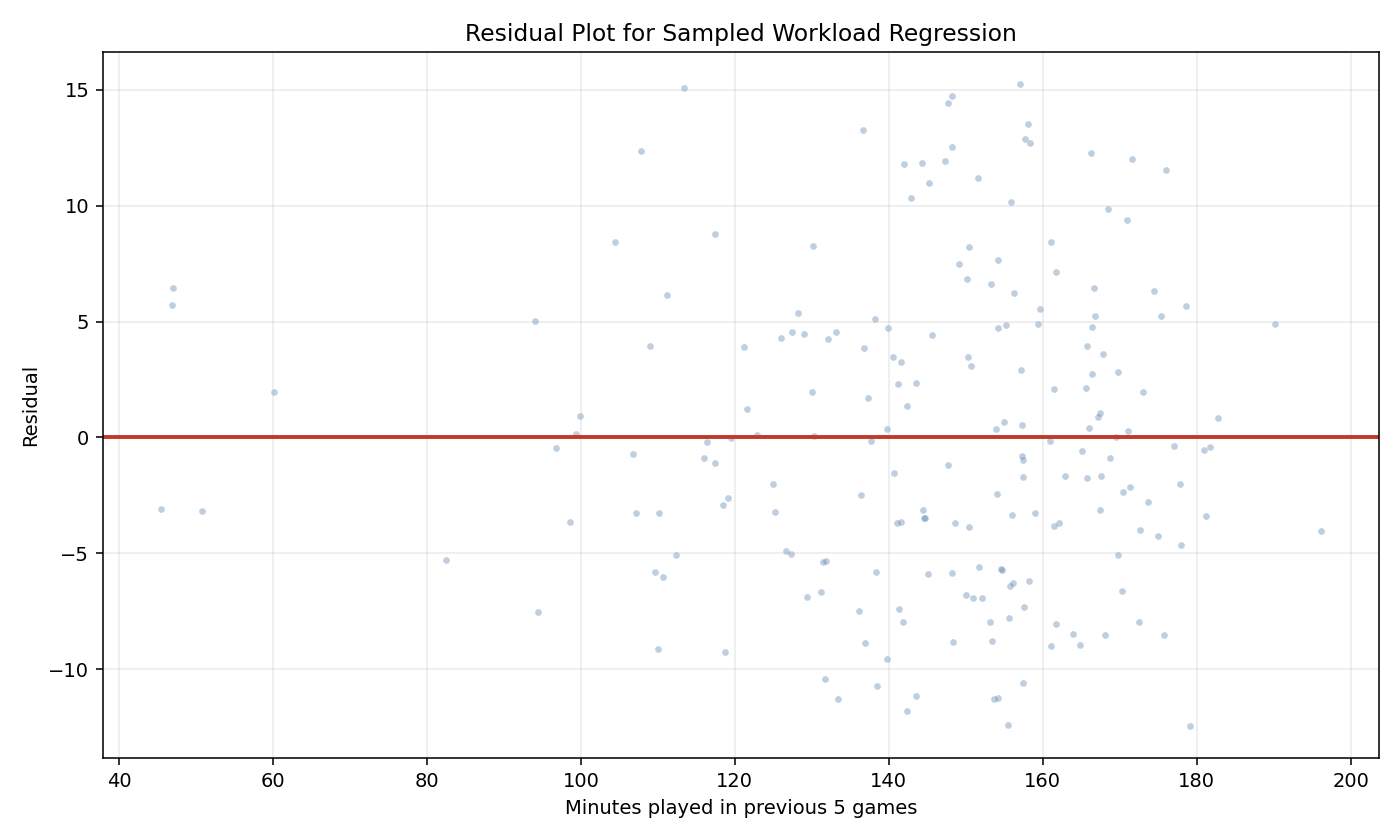
\includegraphics[width=0.82\linewidth]{sampled_residual_plot.png}
\caption{Residual plot for the sampled regression.}
\end{figure}

\subsection*{Independent}

The sample contains 200 player-game observations. Since

\[
200 < 0.10(34,831) = 3,483.1,
\]

the 10\% condition is satisfied. The sampled blocks are non-overlapping within each player-season, so no sampled player-game row is repeated. One limitation is that the five games within a selected block come from the same player-season, so those observations may be somewhat related.

\subsection*{Normal Residuals}

The residual histogram is centered near 0 and does not show extreme skew. The residuals are not perfectly normal, but with $n = 200$, the regression $t$ procedure is reasonably robust.

\begin{figure}[H]
\centering
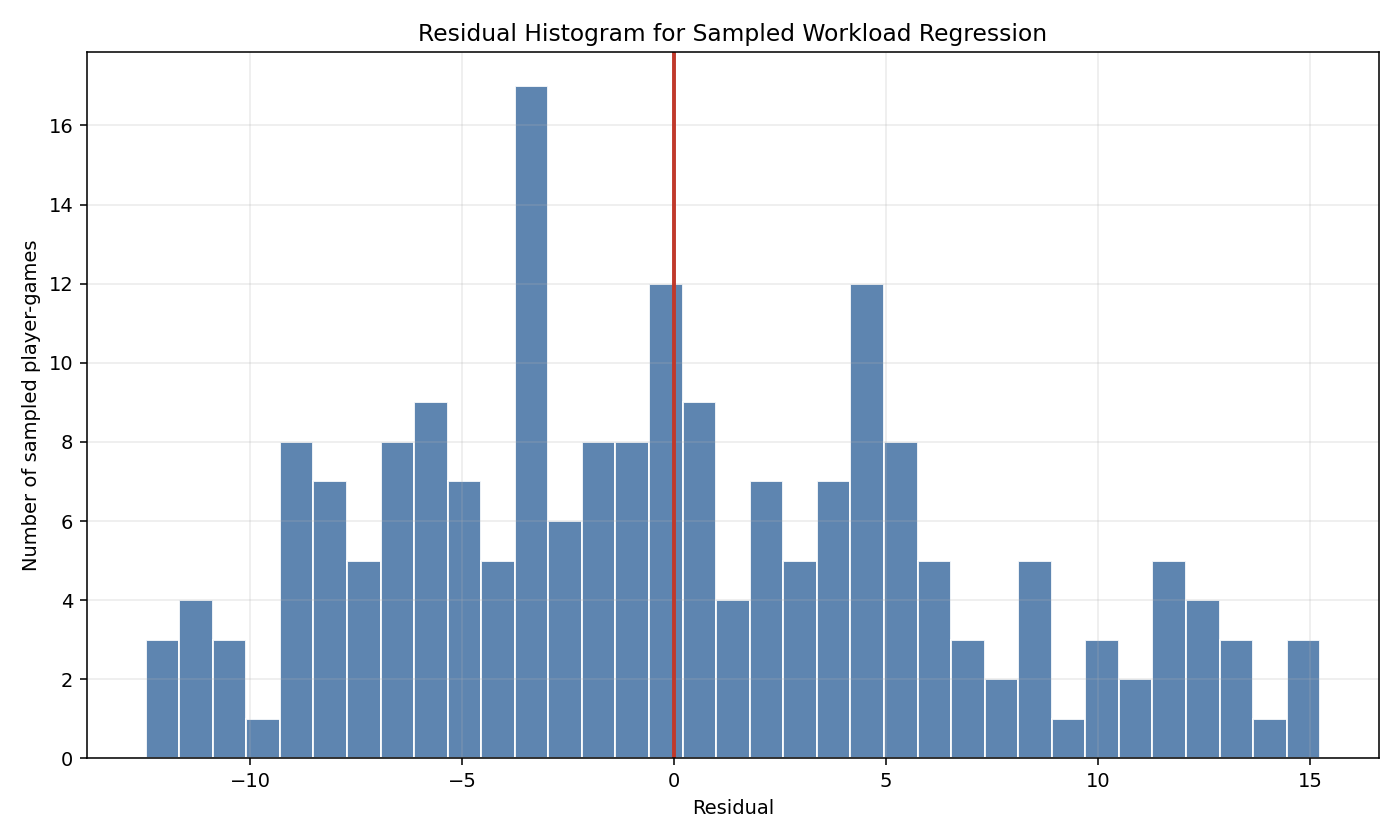
\includegraphics[width=0.82\linewidth]{sampled_residual_histogram.png}
\caption{Histogram of residuals from the sampled regression.}
\end{figure}

\subsection*{Equal Variance}

The residual plot shows residuals scattered around 0 across the range of previous five-game minutes. The spread is not perfectly constant, but there is no severe cone or fan shape, so the equal variance condition is reasonably met.

\subsection*{Random}

The inference data were produced using a random sampling procedure. Player-season strata were randomly selected, and one non-overlapping five-game block was randomly selected from each chosen stratum. A fixed random seed, 2789, was used so the sample can be reproduced.

\section*{Conclusion}

At the $\alpha = 0.05$ significance level, I fail to reject $H_0$. The sample does not provide statistically significant evidence that heavier recent workload is associated with lower current-game Game Score. In fact, the sampled slope is positive, meaning players with more minutes in their previous five games tended to have higher Game Scores in this sample.

This does not prove that fatigue has no effect. The result may be affected by lurking variables. For example, coaches often give more minutes to players who are already playing well, and strong players may both play heavy minutes and earn high Game Scores. However, based on this sample and this regression test, the data do not support the claim that recent workload lowers performance.

\end{document}
